\documentclass[dvipsnames]{article}
\usepackage[utf8]{inputenc}
\usepackage[left=3cm, right=3cm, top=2cm]{geometry}
\title{Dynamic Boundary Conditions}
\author{Silvin Willemsen}
\date{June 2020}

\usepackage{natbib}
\usepackage{graphicx}
\usepackage{appendix}
\usepackage{amsmath}
\usepackage{amsfonts}
\usepackage{amssymb}
\usepackage{subfig}
\usepackage{xcolor}
\def\SBcomment[#1]{\textcolor{red}{#1}}
\def\SWcomment[#1]{\textcolor{blue}{#1}}
\def\SScomment[#1]{\textcolor{green}{#1}}
\def\type[#1]{\textcolor{purple}{#1}}

\begin{document}
\maketitle

\section{Introduction}
This document shows the work done and documentation on dynamic boundary conditions.
 
\section{Explanation}
Let's take the 1D wave equation in discrete time:
\begin{equation}
    \rho A\delta_{tt}u_l^n=T\delta_{xx}u_l^n,
\end{equation}
with simply supported boundary conditions such that
\begin{equation}\label{eq:1Dwave}
u_l^n = \delta_{xx}u_l^n = 0 \quad \text{at} \quad l = 0, N,
\end{equation}
which states that both the state of and the curvature at the boundaries should be 0.

Through stability analysis one can arrive at a condition for the grid spacing that needs to be satisfied in order for the implementation to be stable. In this case this is
\begin{equation}\label{eq:stabilityCondition}
    h \geq ck,
\end{equation}
where wavespeed $c = \sqrt{T/\rho A}$ and time step $k = 1/f_\text{s}$ with sample rate $f_\text{s}$. The closer $h$ is to this condition, the more accurate the scheme will be and the less bandwidth we lose. The reason we can't always satisfy condition \eqref{eq:stabilityCondition} with equality (and consequently utilise the full bandwidth) is due to the fact that we require an integer number of grid points. In other words, we can't use ``fractional grid points". Usually, the following steps are followed to calculate $h$ \cite[Section 6.2.10]{Bilbao2009}:
\begin{equation}
    \qquad N := \text{floor}(1/ck) \qquad h := 1/N.
\end{equation}
There are cases where we can satisfy condition \eqref{eq:stabilityCondition} with equality, such as when using a wavespeed of $c = 1470$ m/s and sample rate $f_\text{s} = 44100$ Hz we can satisfy the stability condition with equality $h = 1/30$ (see Figure \ref{fig:fullString}) . However, this is special case, and if we want to change the wave speed dynamically we need to come up with something smarter. I would like to propose, \textit{interpolated boundary conditions}, the possibility of which has briefly been mentioned by Stefan Bilbao in a footnote \cite[p. 145]{Bilbao2009}, but never elaborated on\footnote{...as "Footnotes are usually written by people who are pretending to know something but actually don't!" -- Bilbao, 2020.}. 
\begin{figure}[h]
    \centering
    \subfloat[String $N=30$.]{\label{fig:fullString}{ 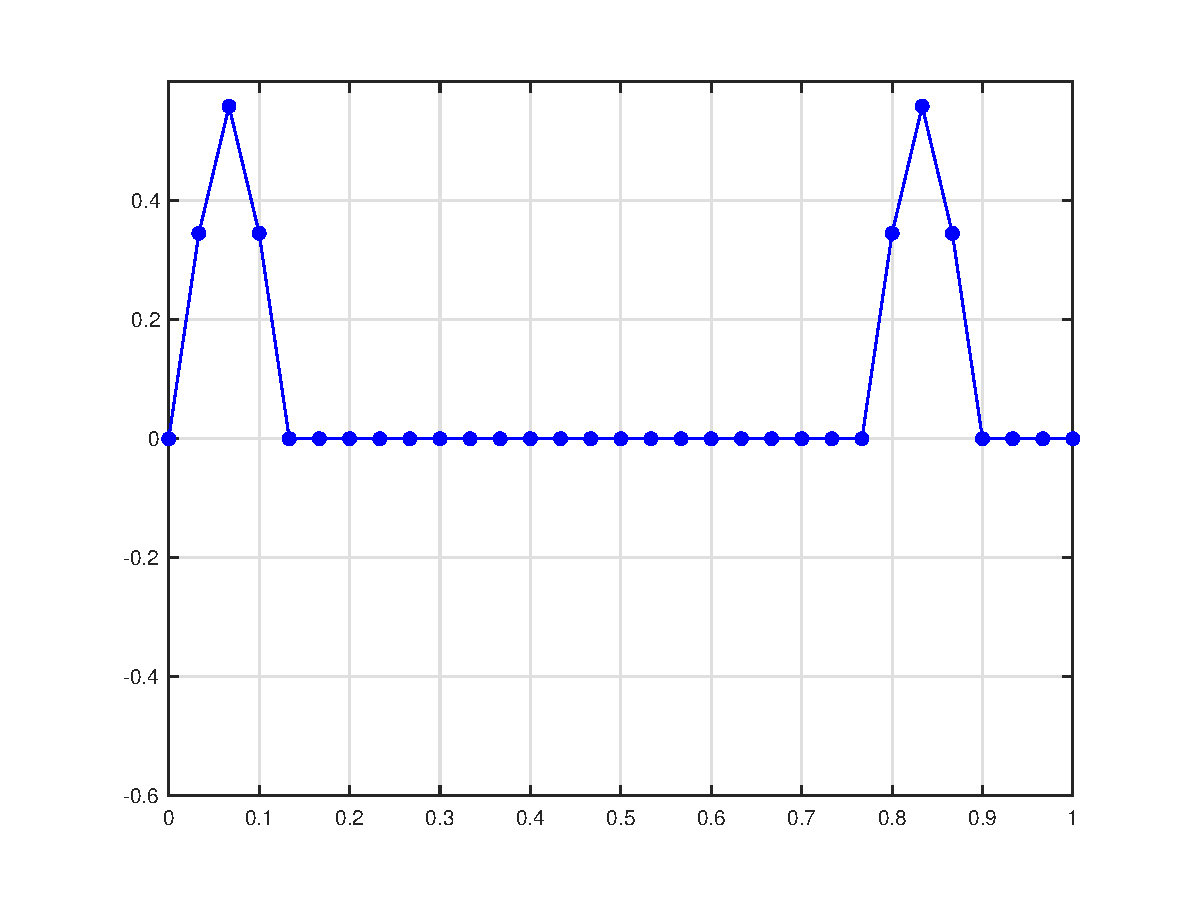
\includegraphics[width=0.33\textwidth]{plot1.eps}}}
    \subfloat[At the left boundary.]{\label{fig:leftBoundary}{ 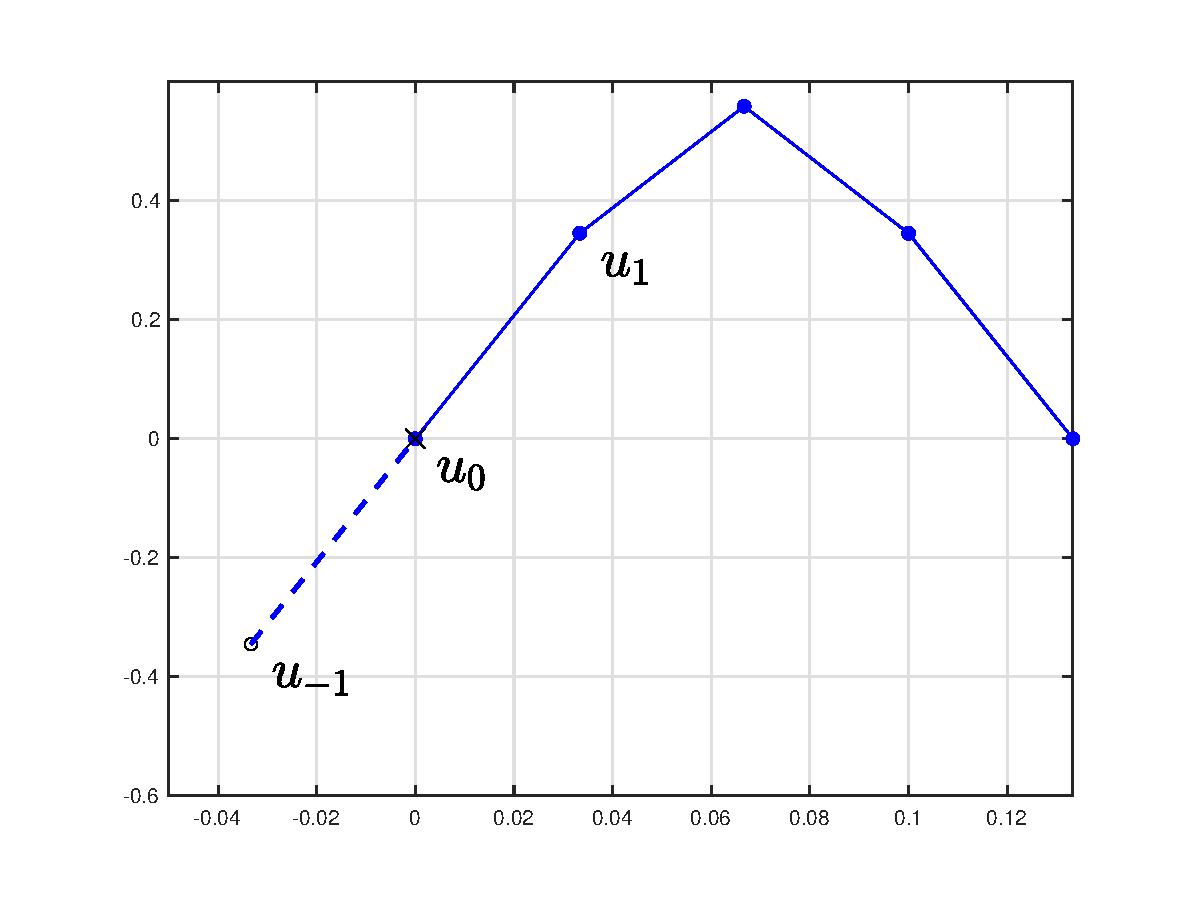
\includegraphics[width=0.33\textwidth]{plot2.eps}}}
    \subfloat[Curvature at the boundary (in this case at $u_0$) should be 0.]{\label{fig:boundaryCondition}{ 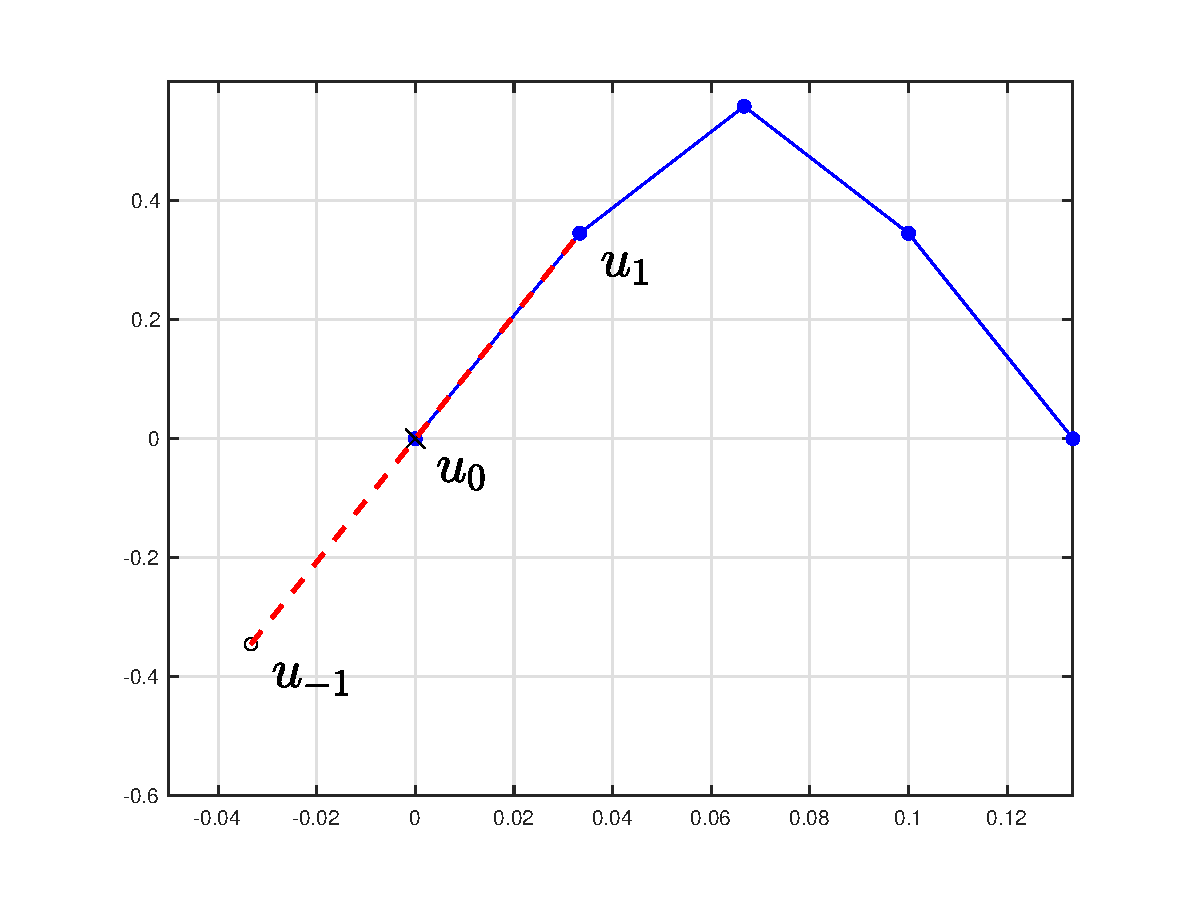
\includegraphics[width=0.33\textwidth]{plot3.eps}}}
    \caption{Case of grid point on boundary.}
\end{figure}

\begin{figure}[h]
\centerline{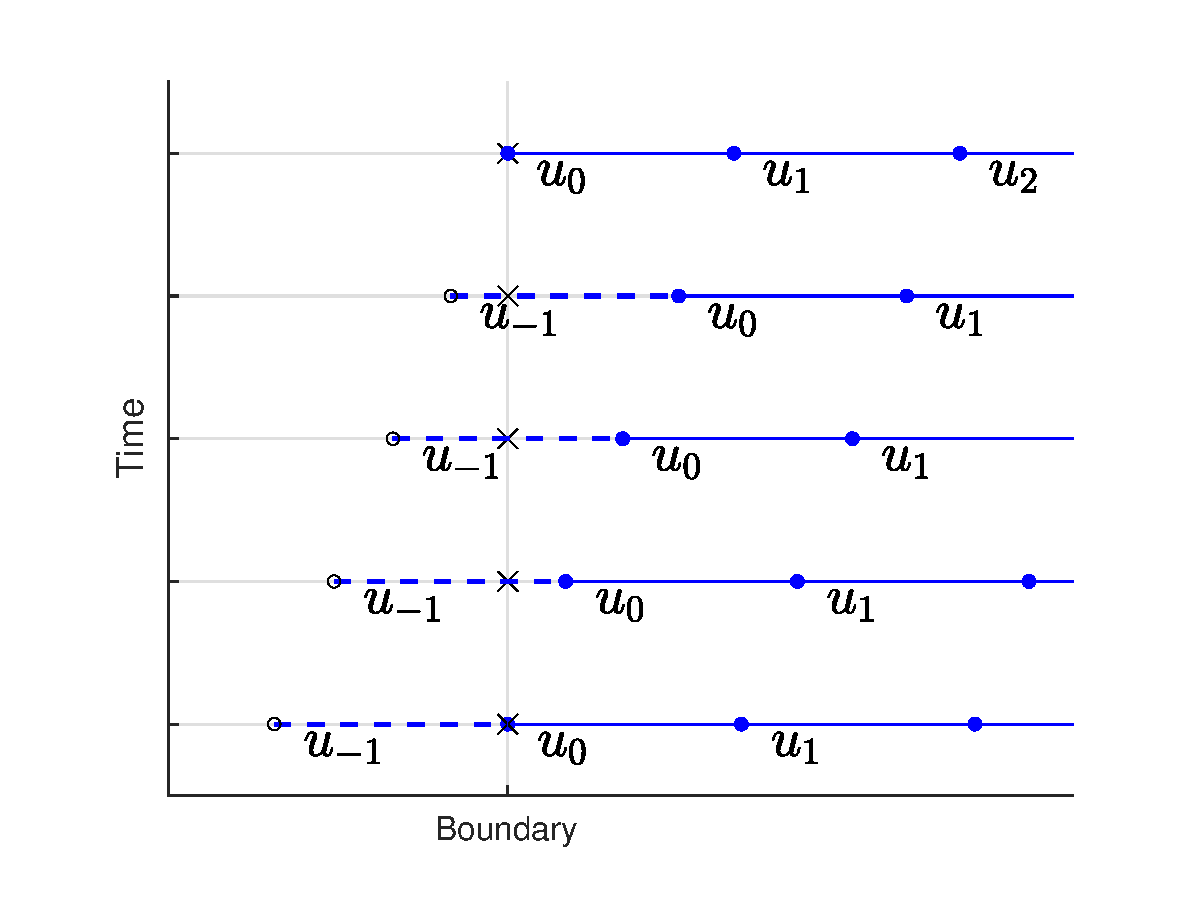
\includegraphics[width=0.6\columnwidth]{dynamic2.eps} }
\caption{\label{fig:dynamicGrid}{Grid changing over time.}}
\end{figure}
\subsection{Analogy with a real-life string}
Imagine detuning a real-life string, or changing the value for tension $T$. If we imagine the tuning knob being at the nut (left boundary), more material will appear on that side when $T$ decreases, and vice versa. To make the transition to the finite-difference setting easier, imagine equidistant points drawn on this string in such a way that there is a point exactly at the nut and the bridge (i.e. at each boundary). Then, when decreasing the tension, the point at the nut will start moving towards the bridge. As a matter of fact, all points (except for the one at the bridge) will start moving towards the bridge! Effectively, we slowly decrease the space between the points which in finite-difference setting is analogous to decreasing the grid spacing $h$. If we do this according to condition \eqref{eq:stabilityCondition}, we get the great side-effect of always satisfying this condition with equality, which means that we don't lose accuracy (or bandwidth). The issue left to solve now is to figure out what to do around the boundary. We continue by still satisfy the boundary condition: the curvature around the boundary needs to be $0$. 
% \begin{figure}[h]
% \centerline{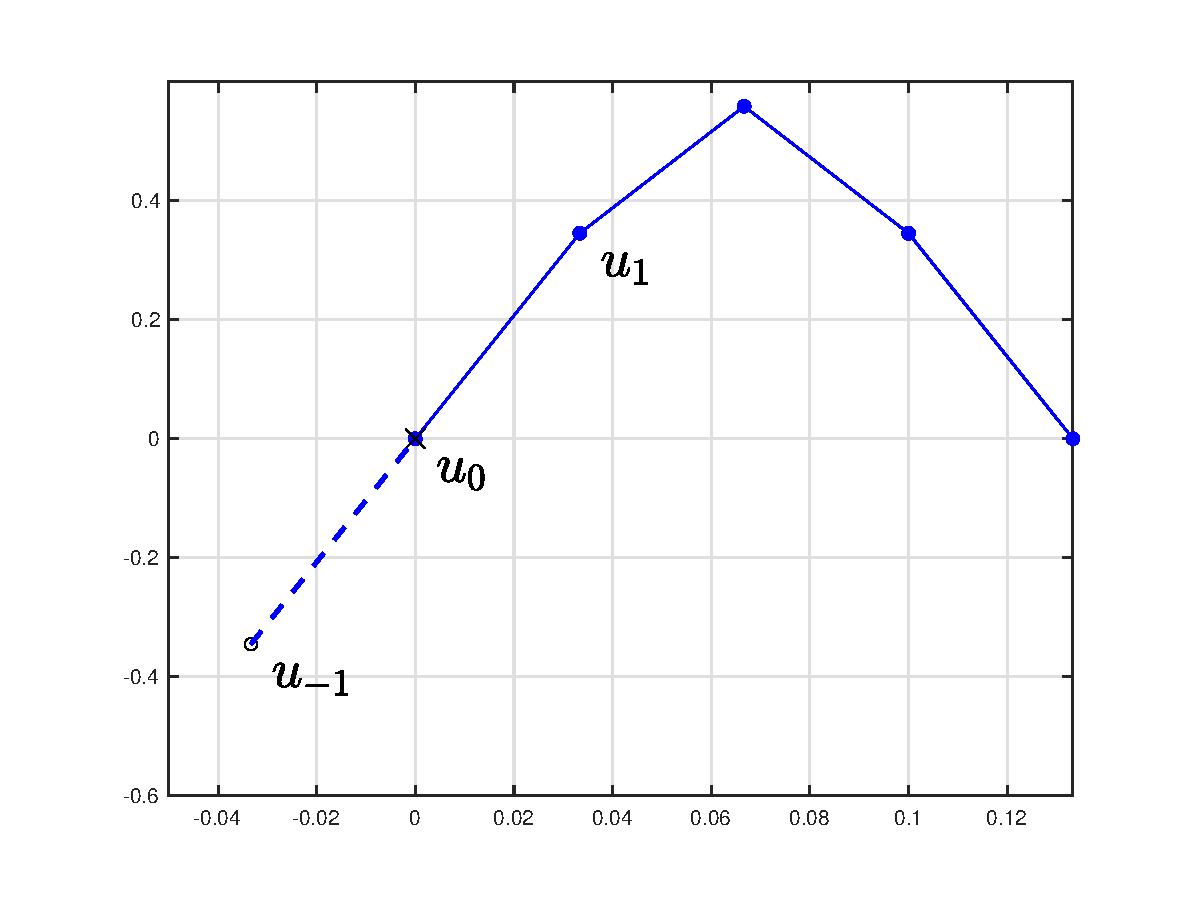
\includegraphics[width=0.6\columnwidth]{plot2.eps}}
% \caption{\label{fig:eta}{At the left boundary.}}
% \end{figure}

% \begin{figure}[h]
% \centerline{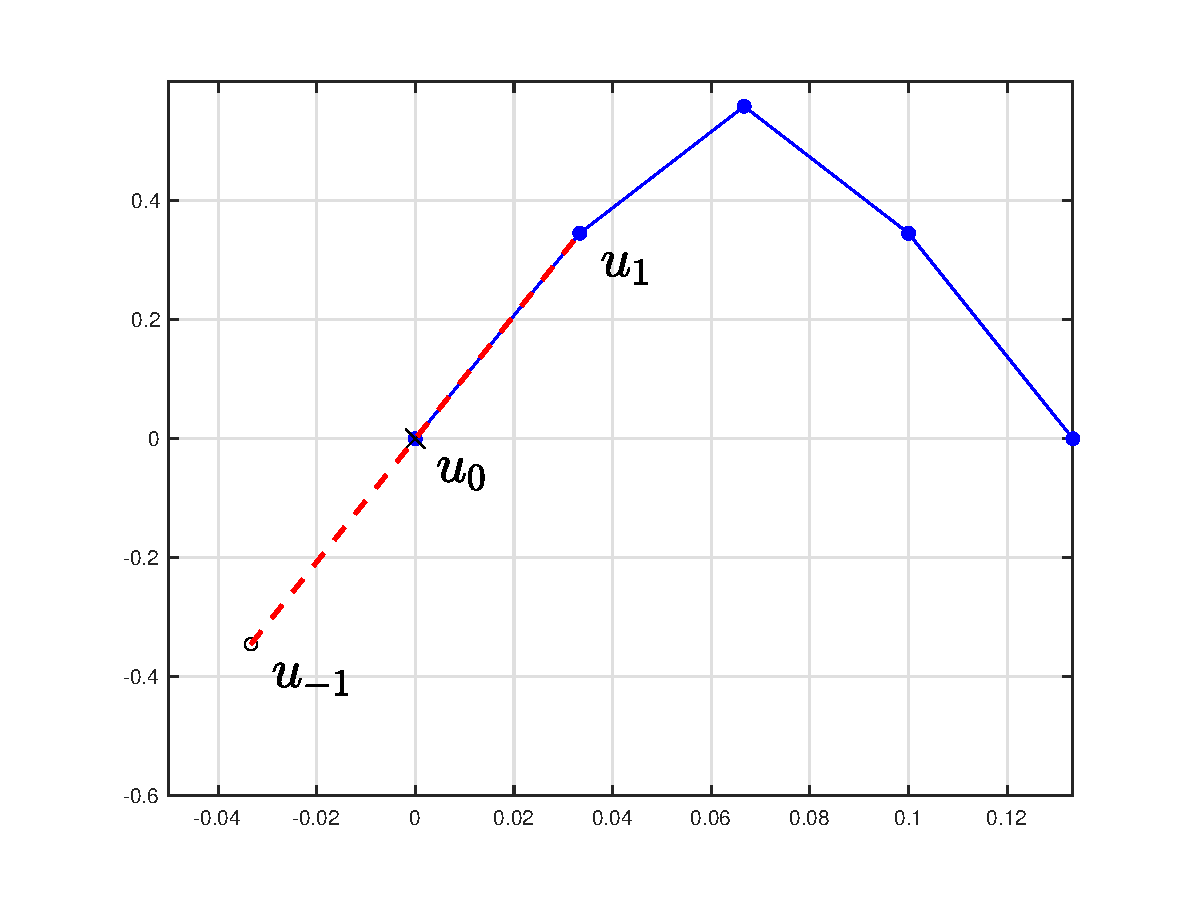
\includegraphics[width=0.6\columnwidth]{plot3.eps}}
% \caption{\label{fig:eta}{Boundary Condition. Curvature at $u_0$ needs to be 0.}}
% \end{figure}

\section{Energy}
We can get the energy of Eq. \eqref{eq:1Dwave} by first taking the inner product with respect to $\delta_{t\cdot}u$ like
\begin{equation}
    \delta_{t+}\mathfrak{h} = \rho A\langle \delta_{t\cdot}u, \delta_{tt}u\rangle_\mathcal{D} - T \langle \delta_{t\cdot}u,\delta_{xx}u\rangle_\mathcal{D} = 0,
\end{equation}
using integration by parts to get
\begin{equation}\label{eq:innerProd}
    \delta_{t+}\mathfrak{h} = \rho A\langle \delta_{t\cdot}u, \delta_{tt}u\rangle_\mathcal{D} + T \langle \delta_{t\cdot}\delta_{x+}u,\delta_{x+}u\rangle_{\underline{\mathcal{D}}} = \mathfrak{b},
\end{equation}
where boundary term
\begin{equation}
    \mathfrak{b} = T (\delta_{t\cdot}u_N)(\delta_{x+}u_N) - T(\delta_{t\cdot}u_0)(\underbrace{\delta_{x+}u_{-1}}_{\delta_{x-}u_0})\ .
\end{equation}
Expanding Eq. \eqref{eq:innerProd} yields,
\begin{equation}
    \delta_{t+}\mathfrak{h} = \rho A \sum_\mathcal{D}h(\delta_{t\cdot}u)(\delta_{tt}u) + T \sum_{\underline{\mathcal{D}}}(\delta_{t\cdot}\delta_{x+}u)(\delta_{x+}u)
\end{equation}
Then, we can finally obtain the energy $\mathfrak{h}$ using the following identities  
\begin{equation}
    (\delta_{t\cdot}u)(\delta_{tt}u) = \delta_{t+}\left(\frac{1}{2}(\delta_{t-}u)^2\right) \quad \text{and} \quad (\delta_{t\cdot}u)u = \delta_{t+}\left(\frac{1}{2}u e_{t-}u\right)
\end{equation}

\begin{gather}
        \mathfrak{h} = \mathfrak{t} + \mathfrak{v}\quad \text{where}\\
    \mathfrak{t} = \frac{\rho A}{2} \sum_{\mathcal{D}} h (\delta_{t-}u_l^n)^2 \quad \text{and} \quad \mathfrak{v} =  \frac{T}{2}\sum_{\underline{\mathcal{D}}}h (\delta_{x+}u_l^n)(\delta_{x+}u_l^{n-1})
\end{gather}

\subsection{Issue regarding increasing $T$}
When the string is already moving and we increase the tension $T$ (moving from top to bottom in Figure \ref{fig:dynamicGrid}), $u_0$ will be moving due to its inertia ($\rho A \delta_{tt}u$). 
\bibliographystyle{plain}
\bibliography{bibliography}
\end{document}
